\section {Data and initial analysis}

\subsection{Data Set}
Our data set is provided by China Telecom. It contains a record of
user information, a historical visiting records to video platforms,
and a dictionary of videos. 

\para {User information.}  China Telecom provides us xxx records of
wired cable users in Shanghai. Each user has a unique identifier, and
the longitude and latitude coordinates of her home address. Since the
Internet is cabled, we can consider the provided location is the exact
location where users watch the videos. This information allows us to
conduct fine-grained study on the preference consistence of users in
nearby areas.

\para {Visiting history.} We are also provided with a video watch
history from \fixme{xxx} users between \fixme{ 2014xxxx to 2014xxxx}. This record
contains user ID, timestamp, device information (desktop or mobile,
os, and device type), and video
information (video source, name, and category). Multiple clicks on
the same video is distinguished in our data set. 

\para {Video dictionary.} The video dictionary contains information
for all videos that users watch. It contains an ID, the source of
platform, name, and categories. The videos in our data set come from 6
large video platforms in China, including Youku and Iqiyi. This allows
us to explore if users have common interests across different
platforms.



\subsection{Data Clean}

\para{Limitations.} Though the data is rich and comprehensive, it has
several limitations. First, there are some fraud clicks in the
data. Some videos have the intention to gain (fake) pageviews. As a
result, there could be some machines to click the video
repeatedly. Second, a lot of videos (\fixme{ about xxx}) are not
associated with a category in the orignial data. Finally, different
platforms may have identical videos. To fairly evaluate user behavior
on a video, we also need to identify and merge these identical videos.


\para{ Fraud users.} We first explain how we detect and remove the
fraud users. 

\para{Video category.}

\para{Unique videos.}


\subsection{Initial Analysis}
\begin{figure*}[t]
% \begin{minipage}{0.32\textwidth}
%  \centering
% 	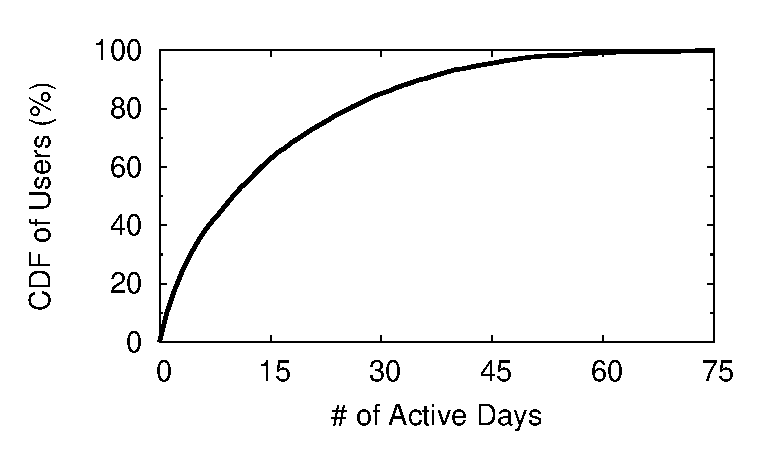
\includegraphics[width=1\textwidth]{plots/basic/cdf_user_active_days.eps}
% 	\caption{Distribution of user active days.}
% 	\label{fig:cdf_active_user}
% \end{minipage}
% \hfill
% \begin{minipage}{0.32\textwidth}
%  \centering
% 	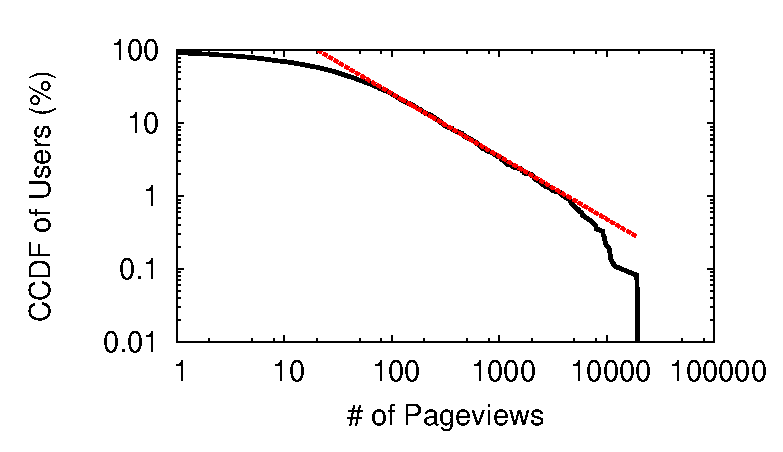
\includegraphics[width=1\textwidth]{plots/basic/ccdf_user_pageviews.eps}
% 	\caption{Distribution of user pageviews.}
% 	\label{fig:ccdf_user_pv}
% \end{minipage}
% \hfill
\begin{minipage}{0.32\textwidth}
 \centering
	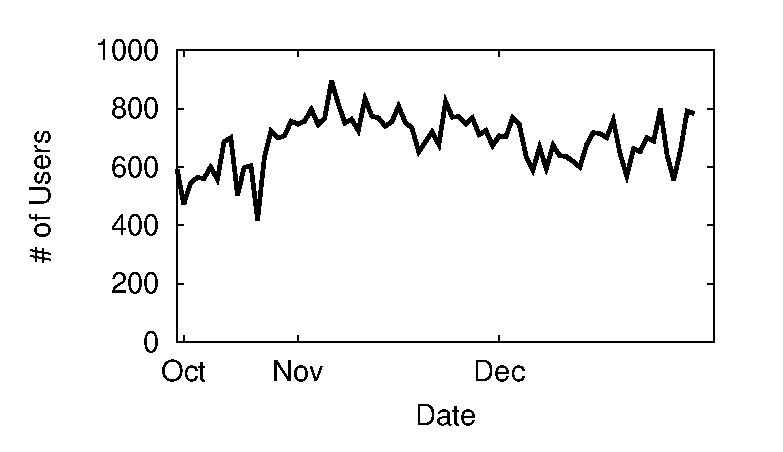
\includegraphics[width=1\textwidth]{plots/basic/dynamic_by_day.eps}
	\caption{User dynamics across days.}
	\label{fig:user_dynamic_day}
\end{minipage}
\end{figure*}

\begin{figure*}[t]
\begin{minipage}{0.32\textwidth}
 \centering
	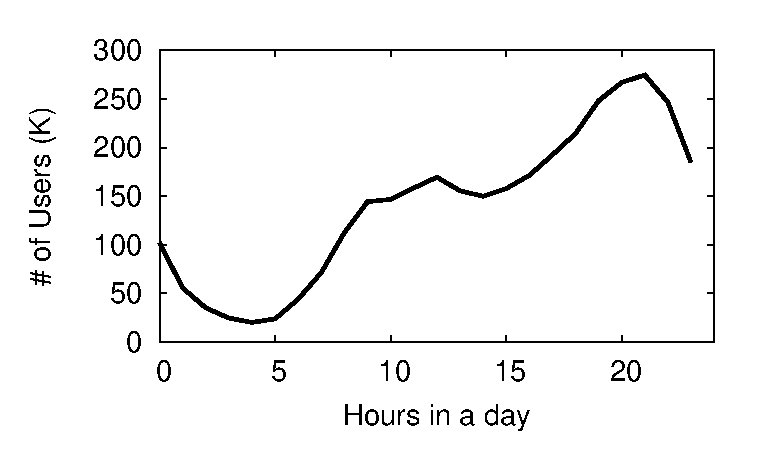
\includegraphics[width=1\textwidth]{plots/basic/dynamic_by_hour.eps}
	\caption{User dynamics in a day.}
	\label{fig:user_dynamic_hour}
\end{minipage}
\hfill
\begin{minipage}{0.32\textwidth}
 \centering
	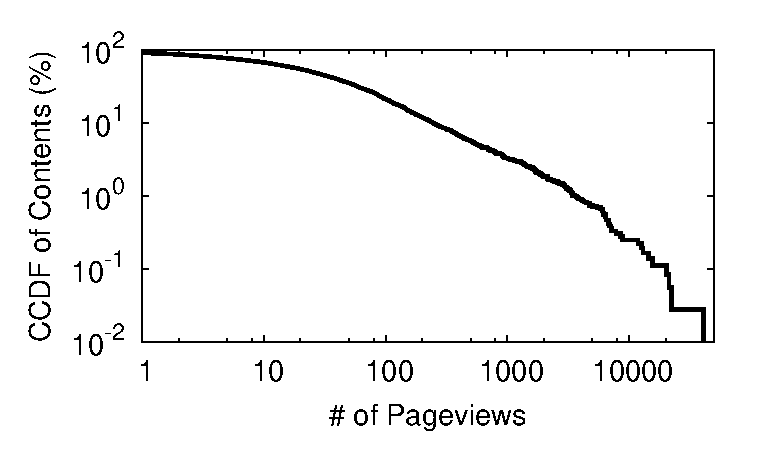
\includegraphics[width=1\textwidth]{plots/basic/ccdf_content_pageviews.eps}
	\caption{Distribution of video pageviews.}
	\label{fig:cdf_content_pv}
\end{minipage}
\hfill
\begin{minipage}{0.32\textwidth}
 \centering
	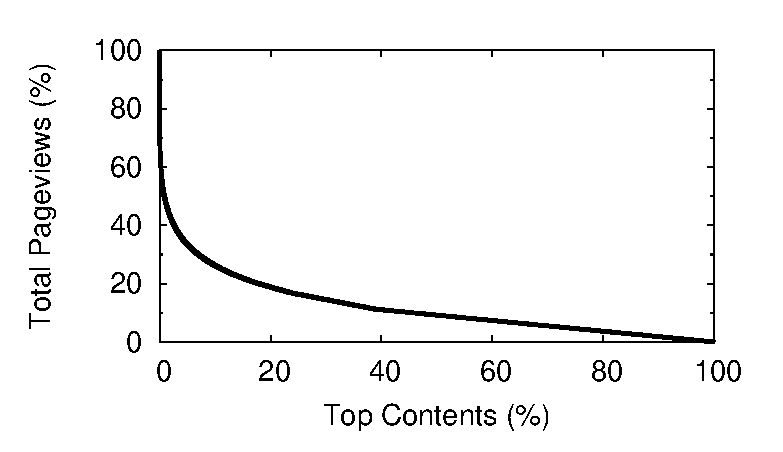
\includegraphics[width=1\textwidth]{plots/basic/top_video_pageviews.eps}
	\caption{Contribution of top videos to total pageviews.}
	\label{fig:top_video_pv}
\end{minipage}

\end{figure*}